\chapter[Metodologia]{Metodologia}
\label{cap:metodologia}
Este capítulo irá abordar a metodologia utilizada no desenvolvimento deste trabalho, discorrendo sobre as metodologias de pesquisa e desenvolvimento, requisitos, arquitetura, ferramentas tecnológicas, cronograma de atividades e a simulação realizada para validação da arquitetura, disponível no Apêndice X.

\section[Metodologias]{Metodologias}
\label{sec:metodologia-proposta}
\subsection[Metodologia de Pesquisa]{Metodologia de Pesquisa}
Conforme descrito na Seção \ref{sec:metodologia}, uma metodologia de pesquisa pode ser classificada com relação à sua abordagem, natureza, objetivo e procedimentos. Cada umas dessas características da pesquisa realizada neste trabalho é descrita a seguir.

\subsubsection[Abordagem da Pesquisa]{Abordagem da Pesquisa}

A pesquisa qualitativa se preocupa com o aprofundamento da compreensão de um grupo social, buscando explicar o por quê das coisas, sem se preocupar com representativades numéricas, e sim com aspectos da realidade que não podem ser quantificados, como significados, motivos, aspirações, crenças, valores e atitudes \cite{gerhardt2009metodos}.

Tendo em vista que a pesquisa realizada foi feita com o objetivo de se compreender o que é gamificação, sistemas de recomendação e o potencial da aprendizagem quando se aprende com uma pessoa mais experiente em uma área do saber, a abordagem da pesquisa se qualifica como qualitativa.

\subsubsection[Natureza da Pesquisa]{Natureza da Pesquisa}

A pesquisa aplicada tem como objetivo gerar conhecimentos para aplicação prática, dirigidos à solução de problemas específicos \cite{gerhardt2009metodos}.

A pesquisa realizada teve o objetivo de obter conhecimentos sobre gamificação, sistemas de recomendação, entre outros conceitos, para a criação de uma aplicação web para mitigação de dificuldades de aprendizagem.

\subsubsection[Objetivo da Pesquisa]{Objetivo da Pesquisa}

A pesquisa exploratória tem como objetivo proporcionar maior familiaridade com o problema, com a finalidade de torná-lo mais explícito ou de constituir hipóteses. Pode-se dizer que seu objetivo principal é o aprimoramento de ideias ou a descoberta de intuições. Na maioria dos casos envolvem levantamento bibliográfico \cite{gil2002elaborar}.

A pesquisa objetivou encontrar referências bibliográficas para levantar a hipótese do sucesso que a aplicação web desenvolvida poderia alcançar.

\subsubsection[Procedimento da Pesquisa]{Procedimento da Pesquisa}

A pesquisa bibliográfica é feita a partir do levantamento de referências teóricas já analisadas e publicadas por meios escritos e eletrônicos, como livros, artígos científicos e páginas de \textit{websites} \cite{gerhardt2009metodos}. Embora em quase todos os estudos seja exigido algum tipo de trabalho dessa natureza, a pesquisa bibliográfica é desenvolvida exclusivamente a partir de fontes bibliográficas. A principal vantagem dessa pesquisa reside no fato de permitir ao investigador a cobertura de uma gama de fenômenos muito mais ampla do que aquela que poderia pesquisar diretamente \cite{gil2002elaborar}.

A pesquisa levantou somente material bibliográfico publicado em livros ou meios eletrônicos, se baseando unicamente em fontes desse tipo para coletar informações.

\subsection[Metodologia de Desenvolvimento]{Metodologia de Desenvolvimento}
\label{metodologia-desenvolvimento}

Para a condução deste trabalho, foi adotada uma Metodologia de Desenvolvimento de Software adaptada, que combina práticas do XP e do \textit{Kanban}. Essa abordagem se deve à realidade da equipe, composta por apenas dois desenvolvedores, para garantir a colaboração e a eficiência do fluxo de trabalho. A seguir, será detalhado cada uma dessas metodologias e as adaptações realizadas para o sucesso do projeto.

\subsubsection[XP]{XP}
A metodologia XP é uma abordagem ágil de desenvolvimento de software que envolve um conjunto de regras e práticas constantes no contexto de quatro atividades metodológicas: planejamento, projeto, codificação e testes \cite{pressman2021engenharia}. Segundo \citeonline{BeckAndres2004} o que distingue o XP de outras metodologias são os seguintes pontos:

\begin{itemize}

\item Ciclos de desenvolvimento curtos, quais geram significados, evidente e contínuo;

\item Técnica de planejamento gradual;

\item Ajustar implementação de funcionalidades de forma flexível para mudanças constantes das necessidades comerciais;

\item Testes automatizados para acompanhar o progresso do desenvolvimento, com intuito de identificar problemas antecipadamente.

\end{itemize}

% \begin{figure}
%     \centering
%     \includegraphics[width=0.5\linewidth]{}
%     \caption{Caption}
%     \label{fig:fluxoAgil}
% \end{figure}

Foram adaptados os seguintes valores e práticas para o contexto deste trabalho: 

\begin{itemize}
    \item \textbf{Comunicação e \textit{Pair Programming}}:
    Dois desenvolvedores trabalham em conjunto em um único computador. Um escreve o código  enquanto o outro revisa, sugere melhorias e pensa estrategicamente. Isso fornece um mecanismo para solução de problemas em tempo real (duas cabeças normalmente funcionam melhor do que uma) e garantia da qualidade em tempo real (o código é revisto à medida que é criado) \cite{pressman2021engenharia}. O papel foi intercalado entre os desenvolvedores.

    \item \textbf{Desenvolvimento Orientado a Testes}:
    A prática de escrever testes automatizados antes de escrever o código funcional que o fará passar nos critérios de aceitação. Os testes automatizados servem como uma documentação do sistema e uma rede de segurança e confiança de que futuras funcionalidades não irão quebrar as funcionalidades já existentes.

    \item \textbf{\textit{Simple Design}}:
    O princípio de projetar a solução mais simples que atenda aos requisitos atuais, evitando \textit{overengineering} e complexidade desnecessária.

    \item \textbf{Entregas Curtas}:
    O ciclo de entregas definido para esse trabalho foi de uma semana. Ao final de cada semana, uma nova versão funcional do software foi gerada. Com a integração contínua simplificada dado o \textit{Pair Programming}, o código foi integrado ao final de cada sessão de trabalho, quando não houve eventualidades, para garantir que a base de código esteja sempre estável e atualizada.
\end{itemize}

\subsubsection[Kanban]{Kanban}
O \textit{Kanban} é uma abordagem que dá suporte a uma metodologia, \textit{framework} ou outra abordagem já existente (no caso deste trabalho, o XP). O \textit{Kanban} tem a intenção de ajudar a gerenciar o trabalho e prestação de serviços ao ponto de atender de maneira consistente as expectativas dos clientes \cite{Bartel2021}.
Segundo \citeonline{pressman2021engenharia} as práticas do \textit{Kanban} são:

\begin{itemize}
  \item \textbf{Visualizar o fluxo de trabalho no quadro Kanban:} O quadro Kanban é dividido em colunas que representam o estágio de desenvolvimento de cada elemento de funcionalidade do software, que a equipe leva da coluna “por fazer” para a “fazendo” e então para a “feito” à medida que o projeto avança.
  
  \item \textbf{Limite de Trabalho em Progresso:} Os desenvolvedores são incentivados a completar a sua tarefa atual antes de iniciarem outra. Isso reduz o tempo de ciclo, melhora a qualidade do trabalho e aumenta a capacidade da equipe de fornecer funcionalidades de software com maior frequência.
  
  \item \textbf{Gerenciamento de Fluxo:} Reduz os desperdícios por meio do entendimento do fluxo de valor atual, pela análise dos pontos em que sofre interrupções, pela definição de mudanças e pela implementação subsequente dessas mudanças. 
\end{itemize}

\section[Requisitos]{Requisitos}
\label{requisitos}

Os requisitos de um sistema são descrições do que o sistema deve fazer, os serviços que oferece e as suas restrições de funcionamento \cite{sommerville2011engenharia}.

A elicitação de requisitos foi conduzida por meio do método \textit{Lean Inception} \cite{caroli2018lean}. Este método consiste em um \textit{workshop} colaborativo que combina um conjunto de atividades estruturadas, como a definição de personas e o \textit{brainstorming} de funcionalidades, para guiar a equipe na definição do escopo de um Produto Mínimo Viável (MVP), que corresponde a uma versão simples do produto que possui valor para os seus usuários. O modelo do \textit{Lean Inception} é apresentado no Apêndice \ref{lean-inception}.

\subsection[Personas]{Personas}

As Personas são personagens fictícios criados para representar diferentes tipos de usuários que possam vir a utilizar um serviço, produto ou site. Criar personas ajuda a entender melhor as necessidades, experiências, comportamentos e objetivos do seus usuários \cite{dam2019personas}.

Foram criadas duas personas para representar os diferentes perfis de usuários da aplicação: um estudante, que precisa de alguém para o auxiliar no aprendizado de um \textit{hobby}, e um professor particular, que busca expandir sua clientela. No Apêndice \ref{personas} deste trabalho podem ser observadas tais personas. 

\subsection[Benchmarking]{Benchmarking}

Segundo \citeonline{benchmarking}, \textit{benchmarking} é um processo de pesquisa contínuo no qual uma organização realiza comparações de seus produtos, processos e práticas com os de concorrentes, com o propósito de aprimoramento organizacional.

A fim de se identificar quais são as funcionalidades e pontos positivos fornecidos por aplicações concorrentes ao software desenvolvido, foi realizado um \textit{benchmarking} competitivo (caracterizado pelo estudo de concorrentes diretos) de três plataformas: Profes, Superprof e Aloprof. Os resultados podem ser visualizados na Tabela \ref{tab:benchmarking}.

\newpage

\begin{table}[h!]
    \centering
    \caption{\textit{Benchmarking} das Plataformas.} % Ajustei o título para condizer com o conteúdo (estava "Bugs")
    \label{tab:benchmarking}
    
    % A coluna X ajusta a largura. O comando abaixo define um alinhamento melhor para listas.
    \begin{tabularx}{\linewidth}{|l|X|}
        \hline
        \textbf{Nome} & \textbf{Funcionalidades} \\
        \hline
        Profes & 
        \begin{itemize}[nosep, leftmargin=*, after=\vspace{\baselineskip}]
            \item Busca de tutores por área de conhecimento e subáreas específicas.
            \item Filtros de pesquisa por preço por aula e localização geográfica.
            \item Possibilidade de submissão de tarefas e exercícios por parte do aprendiz para resolução assíncrona pelo tutor.
            \item Inteligência artificial própria para auxiliar no aprendizado.
            \item Sistema de avaliação de tutores com nota e comentário.
            \item Exibição da quantidade de avaliações, horas aula e exercícios resolvidos no perfil.
            \item Possibilidade de conversar com o tutor por chat de mensagens.
            \item Envio de notificações de eventos (mensagem nova, avaliações, etc.).
        \end{itemize}  
        \\
        \hline
        Superprof & 
        \begin{itemize}[nosep, leftmargin=*, after=\vspace{\baselineskip}]
            \item Busca de tutores por área de conhecimento e subáreas específicas.
            \item Filtros de pesquisa por preço, localização e nível da aula.
            \item Sistema de avaliação de tutores com nota e comentário.
            \item Envio de notificações na ocorrência de eventos (mensagem nova, pedidos de aula, etc.).
        \end{itemize}
        \\
        \hline
        Aloprof &
        \begin{itemize}[nosep, leftmargin=*, after=\vspace{\baselineskip}]
            \item Busca de tutores por área de conhecimento e subáreas específicas.
            \item Agendamento de sessão de tutoria (que deve ser aceita pelo tutor).
            \item Filtros de pesquisa por preço por aula e localização geográfica.
        \end{itemize}  
        \\
        \hline
    \end{tabularx}
    \vspace{0.1cm}
    
     Fonte: Autoria Própria.
\end{table}

Através do \textit{benchmarking} foi possível notar funcionalidades em comum, como filtros de pesquisa, sistema de avaliação de tutores e envio de notificações na ocorrência de determinados eventos. Vale notar que o software desenvolvido neste trabalho se destaca dos concorrentes por ser o único que utiliza elementos de gamificação.

\subsection[Histórias de Usuário]{Histórias de Usuário}
\label{historias-usuario}

História de Usuário (do inglês \textit{User Story}, abreviado como US) é uma técnica que
descreve uma funcionalidade (F) valiosa para um usuário ou comprador de um sistema ou software. Cada história de usuário possui um ou mais critérios de aceitação (CA), que são condições que devem ser satisfeitas para que a história possa ser considerada concluída na implementação desejada \cite{cohn2004user}. As histórias de usuário foram usadas para fracionar as funcionalidades resultantes do \textit{Lean Inception}.

\newpage

\textbf{Funcionalidades:}

\begin{itemize}
\item \textbf{Autenticação - F01}: Essa funcionalidade permite ao usuário efetuar a conexão (\textit{login}) e desconexão (\textit{logout}) na aplicação.

\item \textbf{Gerenciamento de Perfil - F02}: Essa funcionalidade permite ao usuário editar suas informações, assim como apagar seu perfil da aplicação.

\item \textbf{Agendamento de Tutorias - F03}: Essa funcionalidade permite ao aprendiz agendar uma sessão de tutoria com um tutor da aplicação.

\item \textbf{Sistema de Avaliação - F04}: Permite que aprendizes e tutores forneçam \textit{feedback} mútuo (nota e comentário) após uma sessão de tutoria.

\item \textbf{Comunicação - F05}: Essa funcionalidade permite comunicação mútua entre tutores e aprendizes diretamente pela aplicação através de mensagens.

\item \textbf{Busca e Recomendação de Tutores - F06}: Essa funcionalidade permite ao aprendiz buscar por tutores em áreas que possui interesse de obter tutoria, recebendo recomendação de tutores pela aplicação.

\item \textbf{Sistema de Gamificação - F07}: Esta funcionalidade engloba todos os elementos de \textit{games} da plataforma, como sistemas de pontos, níveis, conquistas e rankings, visando aumentar o engajamento dos usuários.

\end{itemize}

\textbf{Histórias de Usuário do Trabalho:}

\begin{itemize}

\item \textbf{F01 - US01}: Eu, como tutor ou aprendiz, desejo realizar \textit{login} na aplicação para conseguir utilizar suas funcionalidades.

\begin{itemize}

\item \textbf{CA01}: O usuário pode realizar \textit{login} com e-mail e senha.

\item \textbf{CA02}: Em caso de \textit{login} bem-sucedido, o usuário deve ser redirecionado para a página inicial do software.

\item \textbf{CA03}: Em caso de falha na autenticação por e-mail e senha, o software deve exibir uma mensagem genérica de erro, como ``E-mail ou senha inválidos.'', sem especificar qual dos dois está incorreto por segurança.

\end{itemize}

\item \textbf{F01 - US02}: Eu, como tutor ou aprendiz, desejo recuperar minha senha, para que eu possa voltar a acessar a plataforma.

\begin{itemize}

\item \textbf{CA01}: O usuário deve informar o e-mail para que o sistema localize sua conta.

\item \textbf{CA02}: O software deve gerar um \textit{link} de redefinição de senha que seja único e com tempo de validade limitado.

\item \textbf{CA03}: O software deve enviar um e-mail para o endereço fornecido contendo o \textit{link} de redefinição, caso o e-mail informado pelo usuário corresponda a um e-mail cadastrado no software.

\item \textbf{CA04}: Por razões de segurança, o software deve exibir a mesma mensagem de sucesso na tela (exemplo: ``Se houver uma conta associada a este e-mail, você receberá um \textit{link} para redefinir sua senha.''), independentemente de o e-mail existir ou não na base de dados.

\item \textbf{CA05}: Ao clicar no \textit{link} válido, o usuário deve ser levado a uma nova página do software em que poderá redefinir e confirmar uma nova senha.

\end{itemize}

\item \textbf{F01 - US03}: Eu, como tutor ou aprendiz, desejo alterar minha senha para possuir uma senha mais fácil de memorizar.

\begin{itemize}

\item \textbf{CA01}: O usuário deve informar a senha atual para poder alterá-la.

\item \textbf{CA02}: O usuário deve informar a nova senha duas vezes.

\item \textbf{CA03}: A nova senha deve ser igual em ambas as inserções.

\item \textbf{CA04}: A nova senha deve atender aos critérios de segurança da plataforma (exemplo: mínimo de 8 caracteres, contendo pelo menos uma letra maiúscula e um número).

\item \textbf{CA05}: Após a alteração bem-sucedida, o sistema deve exibir uma mensagem de confirmação para o usuário.

\item \textbf{CA06}: Caso a senha atual informada não corresponda à senha da conta do usuário, o software deve exibir uma mensagem de erro ao usuário (exemplo: ``A senha atual não corresponde à senha dessa conta.'').

\item \textbf{CA07}: Caso o usuário informe duas novas senhas diferentes, o software deve exibir uma mensagem de erro ao usuário (exemplo: ``Duas senhas novas diferentes. Mudança não efetuada.'').

\end{itemize}

\item \textbf{F02 - US04}: Eu, como tutor ou aprendiz, desejo alterar minhas informações básicas para que meu perfil público se mantenha atualizado e confiável.

\begin{itemize}

\item \textbf{CA01}: O software deve permitir que o usuário faça o \textit{upload} de uma nova foto de perfil.

\item \textbf{CA02}: O software deve permitir que o usuário edite seu nome de exibição.

\item \textbf{CA03}: O software deve permitir que o usuário altere sua localização (cidade e estado) a partir de uma lista predefinida.

\item \textbf{CA04}: Após salvar as alterações, todas elas devem ser refletidas imediatamente no perfil do usuário.

\end{itemize}

\item \textbf{F02 - US05}: Eu, como tutor, desejo definir e atualizar minha agenda de horários disponíveis para que os aprendizes saibam quando podem agendar sessões comigo.

\begin{itemize}

\item \textbf{CA01}: O sistema deve prover uma interface onde o tutor possa marcar períodos de tempo como ``disponível''.

\item \textbf{CA02}: A agenda de disponibilidade atualizada do tutor deve ser a única referência utilizada pelo software quando um aprendiz for agendar uma tutoria.

\end{itemize}

\item \textbf{F02 - US06}: Eu, como tutor, desejo gerenciar minha lista de especialidades para controlar em quais buscas de áreas de conhecimento meu perfil deve aparecer.

\begin{itemize}

\item \textbf{CA01}: O tutor deve poder adicionar uma ou mais especialidades ao seu perfil, selecionando a partir de uma lista de áreas de conhecimento predefinida pelo software.

\item \textbf{CA02}: O tutor deve poder remover qualquer especialidade da sua lista de áreas de conhecimento.

\item \textbf{CA03}: O tutor deve ter pelo menos uma especialidade definida para ser considerado um tutor e aparecer nos resultados de busca.

\item \textbf{CA04}: As alterações na lista de especialidades devem ser salvas e refletidas imediatamente no perfil público do tutor.

\end{itemize}

\item \textbf{F03 - US07}: Eu, como aprendiz, quero solicitar um horário na agenda de um tutor para iniciar o processo de agendamento de uma tutoria.

\begin{itemize}

\item \textbf{CA01}: O software deve permitir que um aprendiz selecione um horário marcado como ``disponível'' na agenda pública de um tutor.

\item \textbf{CA02}: Ao confirmar a solicitação, o status do horário na agenda do tutor deve mudar de ``disponível'' para ``pendente de confirmação''.

\item \textbf{CA03}: Um horário com solicitação confirmada não deve estar disponível para outros aprendizes solicitarem.

\item \textbf{CA04}: O tutor deve ser notificado de que recebeu uma nova solicitação de agendamento.

\item \textbf{CA05}: A solicitação deve ter um prazo de validade de 24 horas.

\end{itemize}

\item \textbf{F03 - US08}: Eu, como tutor, quero aceitar ou recusar as solicitações de agendamento que recebo para ter total controle sobre minha agenda e aprendizes.

\begin{itemize}

\item \textbf{CA01}: O tutor deve ter uma área em seu painel em que possa visualizar todas as solicitações de agendamento pendentes (aguardando confirmação).

\item \textbf{CA02}: Para cada solicitação pendente, o tutor deve ter as opções ``Aceitar'' e ``Recusar''.

\item \textbf{CA03}: Se o tutor ``Aceitar'', o status do horário deve mudar de ``pendente'' para ``confirmado'', e o aprendiz deve ser notificado da confirmação.

\item \textbf{CA04}: Se o tutor ``Recusar'', o agendamento é cancelado, o horário volta a ter o status ``disponível'', e o aprendiz deve ser notificado da recusa.

\end{itemize}

\item \textbf{F03 - US09}: Eu, como tutor ou aprendiz, quero que uma solicitação de agendamento termine (expire) automaticamente após 24 horas sem resposta para que os horários não fiquem bloqueados indefinidamente.

\begin{itemize}

\item \textbf{CA01}: O software deve monitorar o tempo de vida de todas as solicitações com status ``pendente''.

\item \textbf{CA02}: Se uma solicitação pendente atingir 24 horas de espera sem resposta, é automaticamente expirada (não confirmada).

\item \textbf{CA03}: Quando uma solicitação expira, o horário correspondente na agenda do tutor deve voltar ao status ``disponível''.

\item \textbf{CA04}: O tutor e aprendiz da solicitação devem ser notificados de que a solicitação expirou por falta de resposta do tutor.

\end{itemize}

\item \textbf{F04 - US10}: Eu, como aprendiz, quero avaliar o tutor após uma sessão de tutoria para compartilhar minha experiência sobre a didática e profissionalismo dele com outros aprendizes.

\begin{itemize}

\item \textbf{CA01}: O software deve habilitar a opção de avaliação para ambos os participantes somente após a data e hora da tutoria agendada terem passado (acontecido).

\item \textbf{CA02}: O aprendiz deve poder atribuir uma nota de 1 a 5 estrelas.

\item \textbf{CA03}: O aprendiz deve ter a opção de escrever um comentário de texto para justificar sua nota (o comentário será opcional).

\item \textbf{CA04}: Uma vez que a avaliação (nota e comentário) é enviada, ela não pode ser editada.

\item \textbf{CA05}: A avaliação só se torna visível para o outro usuário (e no perfil público) após ele também ter deixado sua avaliação, ou após um prazo de 48 horas ter passado (o que ocorrer primeiro).

\end{itemize}

\item \textbf{F04 - US11}: Eu, como tutor, quero avaliar o aprendiz após uma sessão de tutoria para sinalizar seu nível de comprometimento e engajamento, ajudando a manter a comunidade segura.

\begin{itemize}

\item \textbf{CA01}: O software deve habilitar a opção de avaliação para ambos os participantes somente após a data e hora da tutoria agendada terem passado.

\item \textbf{CA02}: O tutor deve poder atribuir uma nota de 1 a 5 estrelas.

\item \textbf{CA03}: O usuário deve ter a opção de escrever um comentário de texto para justificar sua nota (o comentário será opcional).

\item \textbf{CA04}: Uma vez que a avaliação (nota e comentário) é enviada, ela não pode ser editada.

\item \textbf{CA05}: A avaliação só se torna visível para o outro usuário (e no perfil público) após ele também ter deixado sua avaliação, ou após um prazo de 48 horas ter passado (o que ocorrer primeiro).

\end{itemize}

\item \textbf{F04 - US12}: Eu, como tutor ou aprendiz, quero ver a reputação de um tutor ou aprendiz em seu perfil público para me ajudar a decidir se desejo iniciar uma interação com ele.

\begin{itemize}

\item \textbf{CA01}: O perfil do usuário deve exibir a média de todas as notas recebidas.

\item \textbf{CA02}: O perfil deve mostrar o número total de avaliações que compõem a média (exemplo: ``4.8 de 120 avaliações'').

\item \textbf{CA03}: Se um usuário atua como tutor e aprendiz, seu perfil deve exibir claramente duas médias de nota separadas: uma para sua atuação como ``Tutor'' e outra como ``Aprendiz''.

\item \textbf{CA04}: O perfil deve listar os comentários individuais recebidos, junto com a nota correspondente àquele comentário e o nome de quem avaliou.

\end{itemize}

\item \textbf{F05 - US13}: Eu, como aprendiz, quero enviar uma mensagem para um tutor a partir de seu perfil público para tirar dúvidas sobre sua metodologia ou disponibilidade antes de agendar uma tutoria.

\begin{itemize}

\item \textbf{CA01}: O software deve permitir que um aprendiz envie uma mensagem de texto para um tutor a partir do perfil dele.

\item \textbf{CA02}: Toda mensagem enviada deve ser registrada e associada corretamente ao remetente (aprendiz) e ao destinatário (tutor).

\item \textbf{CA03}: O tutor deve ser notificado pelo software sobre o recebimento de uma nova mensagem.

\item \textbf{CA04}: A conversa iniciada deve ser armazenada e permanecer acessível para ambos os participantes em sua respectiva área de mensagens

\item \textbf{CA05}: Um tutor não pode iniciar uma conversa com um aprendiz que nunca o contatou.

\end{itemize}


\item \textbf{F06 - US14}: Eu, como aprendiz, desejo buscar por tutores do software usando filtros específicos para encontrar um tutor que auxilie no meu aprendizado.

\begin{itemize}

\item \textbf{CA01}: O software deve permitir a busca de tutores por uma área de conhecimento.

\item \textbf{CA02}: Os resultados da busca devem poder ser ordenados por nota média de avaliação (do maior para o menor).

\item \textbf{CA03}: Os resultados da busca devem poder ser ordenados por número de tutorias realizadas (do maior para o menor).

\item \textbf{CA04}: O software deve permitir filtrar os resultados por localização, dentro de um raio de distância selecionável pelo usuário.

\item \textbf{CA05}:  O software deve exibir o número total de tutores encontrados que correspondem aos critérios de busca e filtro.

\end{itemize}


\item \textbf{F06 - US15}: Eu, como aprendiz, desejo receber recomendações personalizadas de tutores para descobrir tutores relevantes que talvez eu não encontrasse em uma busca comum.

\begin{itemize}

\item \textbf{CA01}: O software deve me recomendar tutores que são especialistas nas áreas de conhecimento que eu marquei como de meu interesse no meu perfil.

\item \textbf{CA02}: O software deve me recomendar tutores que foram bem avaliados por outros aprendizes que têm um perfil e histórico de tutorias semelhantes ao meu.

\item \textbf{CA03}: A lista de recomendações não deve incluir tutores com quem eu já tive uma tutoria agendada ou que eu tenha avaliado negativamente.

\item \textbf{CA04}: O software deve permitir filtrar os resultados por localização, dentro de um raio de distância selecionável pelo usuário.

\item \textbf{CA05}: As recomendações devem ser apresentadas de forma clara, com o título ``Tutores recomendados para você''.

\item \textbf{CA06}: Para cada tutor recomendado, o software deve, idealmente, fornecer uma breve justificativa para a sugestão (ex: ``Porque você se interessa por Python'' ou ``Popular entre aprendizes com seus interesses'').

\end{itemize}


\item \textbf{F07 - US16}: Eu, como tutor ou aprendiz, desejo conseguir conquistas para me sentir recompensado pelo meu comportamento na aplicação.

\begin{itemize}

\item \textbf{CA01}: A conquista deve possuir título.

\item \textbf{CA02}: A conquista deve possuir descrição do que deve ser feito para obtê-la.

\item \textbf{CA03}: A conquista deve possuir imagem.

\item \textbf{CA04}: Caso a conquista tenha sido obtida, a imagem é exibida em cores.

\item \textbf{CA05}: Caso a conquista não tenha sido obtida, a imagem é exibida em tom de cinza.

\item \textbf{CA06}: O usuário é notificado ao obter uma conquista.

\item \textbf{CA07}: Ao ser obtida, a conquista recompensa o usuário com pontos.

\item \textbf{CA08}: O usuário pode consultar uma lista com todas as conquistas da aplicação, que deve diferenciar claramente as que já foram obtidas das que ainda não foram.

\end{itemize}

\item \textbf{F07 - US17}: Eu, como tutor ou aprendiz, desejo obter níveis no meu perfil para me manter engajado a utilizar o software.

\begin{itemize}

\item \textbf{CA01}: O nível é exibido no perfil do usuário.

\item \textbf{CA02}: A transição de um nível para outro deve seguir uma tabela de progressão predefinida que mapeia faixas de pontuação a cada nível (exemplo: Nível 1: 0-100 pts, Nível 2: 101-300 pts).

\end{itemize}

\item \textbf{F07 - US18}: Eu, como tutor ou aprendiz, desejo obter títulos decorativos no meu perfil para sentir satisfação pessoal.

\begin{itemize}

\item \textbf{CA01}: O título é exibido no perfil do usuário. 

\item \textbf{CA02}: Cada título deve ser desbloqueado ao atingir um nível específico, conforme uma tabela de mapeamento predefinida (exemplo: Nível 10 = ``Iniciante'', Nível 20 = ``Experiente'').

\end{itemize}

\item \textbf{F07 - US19}: Eu, como tutor ou aprendiz, desejo ver o ranking dos melhores tutores por área para identificar os profissionais mais experientes e bem avaliados.

\begin{itemize}

\item \textbf{CA01}: O software deve permitir ao usuário selecionar uma área de conhecimento específica para a qual deseja visualizar o ranking.

\item \textbf{CA02}: Somente tutores que atenderem a um critério mínimo de elegibilidade (exemplo: ter 10 ou mais tutorias concluídas naquela área) podem aparecer no ranking.

\item \textbf{CA03}: Os tutores são classificados por nota média de avaliação em ordem decrescente.

\item \textbf{CA04}: O número total de tutorias realizadas na área deve ser utilizado como critério de desempate.

\item \textbf{CA05}: O ranking deverá exibir um número fixo e predefinido dos melhores tutores (como \textit{Top} 10 ou \textit{Top} 5).

\item \textbf{CA06}: Para cada tutor listado, o sistema deve exibir essas informações: posição no ranking, nome, nota média e número total de tutorias concluídas naquela área.

\item \textbf{CA07}: Se não existirem tutores elegíveis para o ranking de uma área, o software deverá exibir uma mensagem informativa, como ``Ainda não há tutores classificados para esta área''.

\item \textbf{CA08}: Os dados do ranking devem ser atualizados a cada 24 horas para refletir as novas atividades na plataforma.

\end{itemize}

\end{itemize}

\subsection[Requisitos Não Funcionais]{Requisitos Não Funcionais}

Usuários possuem expectativas, geralmente não declaradas, sobre o quão bem o produto deverá funcionar. Tais expectativas incluem o quão fácil é sua utilização, o quão rápido é sua execução, o quão raro são suas falhas e como ele lida com condições inesperadas. Tais características são conhecidas como atributos de qualidade ou requisitos de qualidade, e constituem a maior parte dos Requisitos Não Funcionais (RNFs) de um software \cite{wiegers2013software}.

Conforme \citeonline{wiegers2013software}, RNFs determinam decisões de design e arquitetura, levando a um produto mais satisfatório para os usuários caso sejam listados e considerados durante o desenvolvimento, evitando retrabalho. A fim de evitar retrabalho futuro e também para se desenvolver um software mais satisfatório para os usuários, foram elicitados os seguintes RNFs:

\begin{itemize}

\item \textbf{Usabilidade:}

\begin{itemize}

\item \textbf{RNF01}: O software deve utilizar um conjunto de ícones e assets padronizados;

\item \textbf{RNF02}: O software deve realizar a validação dos formulários, impedindo a submissão de dados inválidos e fornecendo \textit{feedback} visual imediato nos campos incorretos.

\end{itemize}

\end{itemize}

\begin{itemize}

\item \textbf{Reusabilidade:}

\begin{itemize}

\item \textbf{RNF03}: O software deve reutilizar os componentes já criados que se encaixem na tarefa necessária;

\end{itemize}

\end{itemize}


\begin{itemize}

\item \textbf{Segurança:}

\begin{itemize}

\item \textbf{RNF04}: O software deve criptografar a senha dos usuários com algoritmos de hash;

\item \textbf{RNF05}: O software deve utilizar o padrão OAuth2 / JWT (\textit{JSON Web Tokens}) para autenticação na API (\textit{Application Programming Interface});

\item \textbf{RNF06}: O token deve ter tempo de expiração curto.

\item \textbf{RNF07}: Toda a comunicação entre o \textit{frontend} e o \textit{backend} deve ser realizada exclusivamente via protocolo HTTPS (\textit{Hypertext Transfer Protocol Secure}) para garantir a confidencialidade dos dados em tráfego.

\end{itemize}

\end{itemize}

\begin{itemize}

\item \textbf{Interoperabilidade:}

\begin{itemize}

\item \textbf{RNF08}: A API deve exportar automaticamente sua documentação técnica seguindo o padrão OpenAPI 3.0 (\textit{Swagger}).
\end{itemize}

\end{itemize}


\subsection[Priorização dos Requisitos]{Priorização dos Requisitos}
\label{priorizacao-requisitos}

Segundo \citeonline{wiegers2013software}, em cenários de escassez de recursos, como restrições temporais, a priorização de requisitos torna-se essencial para o planejamento do desenvolvimento. Essa prática visa antecipar a implementação de funcionalidades críticas, maximizando a entrega de valor ao negócio dentro das limitações do projeto. Uma técnica usada para este fim é o método MoSCoW, que categoriza os requisitos em quatro níveis de prioridade:

\begin{itemize}

\item \textbf{\textit{Must}}: o requisito deve ser satisfeito para a solução ser considerada um sucesso.

\item \textbf{\textit{Should}}: o requisito é importante e deve ser incluído na solução se possível, mas não é mandatório para o sucesso.

\item\textbf{\textit{Could}}: é uma funcionalidade desejável, mas que pode ser postergada ou eliminada. É implementada somente quando o tempo e recursos permitirem.

\item \textbf{\textit{Won't}}: indica que o requisito não será implementado no momento, mas poderia ser incluído em uma versão futura do software.

\end{itemize}

No contexto deste trabalho, o método MoSCoW foi aplicado para a priorização das US, resultando na classificação apresentada a seguir:




\begin{itemize}

\item \textbf{\textit{Must}}:

\begin{itemize}

\item \textbf{US01 (\textit{Login})} 

\item \textbf{US04 (Alterar Informações)}

\item \textbf{US05 (Definir Agenda)}

\item \textbf{US06 (Gerenciar Especialidades)}

\item \textbf{US07 (Solicitar Horário)}

\item \textbf{US08 (Aceitar e Recusar Solicitação)}

\item \textbf{US10 (Avaliar Tutor)}

\item \textbf{US14 (Buscar Tutores)}

\item \textbf{US15 (Recomendações)}

\item \textbf{US16 (Conquistas)}

\end{itemize}

\end{itemize}

\begin{itemize}

\item \textbf{\textit{Should}}:

\begin{itemize}

\item \textbf{US02 (Recuperar Senha)}

\item \textbf{US03 (Alterar Senha)}

\item \textbf{US11 (Avaliar Aprendiz)}

\item \textbf{US12 (Ver Reputação no Perfil)}

\item \textbf{US17 (Níveis)}

\end{itemize}

\end{itemize}

\begin{itemize}

\item \textbf{\textit{Could}}:

\begin{itemize}

\item \textbf{US09 (Expirar Solicitação)}

\item \textbf{US13 (Enviar Mensagem)}

\item \textbf{US18 (Títulos)}

\end{itemize}

\end{itemize}

\begin{itemize}

\item \textbf{\textit{Won't}}:

\begin{itemize}

\item \textbf{US19 (Rankings)}

\end{itemize}

\end{itemize}


\section [Arquitetura] {Arquitetura}
\label{arquitetura}

A arquitetura deste projeto pode ser visualizada por meio da Figura \ref{fig:RepresentacaoArquitetura}. A representação contém uma ilustração que demonstra os elementos básicos do software desenvolvido neste trabalho.

Esta arquitetura foi projetada para maximizar a eficiência do desenvolvimento, a escalabilidade e a manutenibilidade, adotando padrões distintos e especializados para o \textit{backend} e o \textit{frontend}, com o modelo Cliente-Servidor. 

O \textit{backend} implementa uma variação do padrão \textit{Model-View-Controller} (MVC), conhecida como \textit{Model-View-Serializer} (MVS), utilizando o \textit{framework} Django. O \textit{frontend}, por sua vez, é estruturado como um \textit{Monorepo}, facilitando a gestão e o compartilhamento de código na plataforma Next.js.

\begin{figure}[h!]
    \centering
    \caption{Representação Arquitetural.} 
    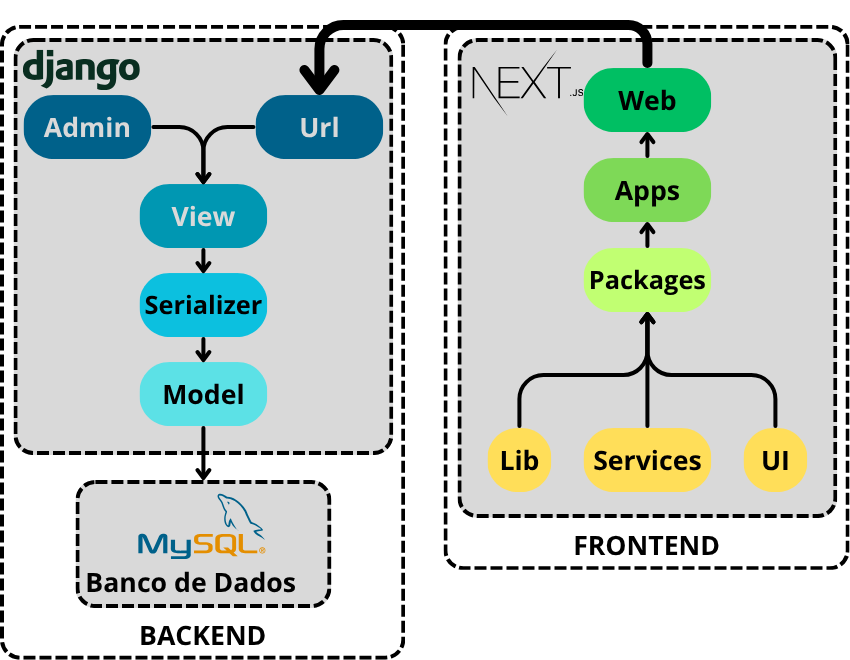
\includegraphics[width=0.70\textwidth]{figuras/Representacao_Arquitetura.png}


    Fonte: Autoria própria.
    
    \vspace{0.2cm}
        
    \label{fig:RepresentacaoArquitetura}
\end{figure}

\subsection [Backend Django]{Backend Django}
O \textit{backend} é responsável pela lógica de negócio, processamento de dados e persistência, seguindo a arquitetura MVS do Django, que promove uma clara separação de responsabilidades.

\textit{Model}: A camada \textit{Model} representa a estrutura dos dados da aplicação. Implementada através das \textit{Models} do Django, ela serve como a única fonte da verdade para os dados. Utilizando o ORM (\textit{Object-Relational Mapping}) integrado do Django, as classes Python são mapeadas diretamente para as tabelas no banco de dados MySQL neste projeto. Toda a lógica de acesso, validação e manipulação dos dados reside aqui.

\textit{View}: Na terminologia do Django, a \textit{View} atua como a \textit{Controller} do padrão MVC clássico. É a camada que processa as requisições HTTP (\textit{Hypertext Transfer Protocol}) recebidas do cliente. Ela contém a lógica de negócio, interage com a \textit{Model} para buscar ou modificar dados e retorna uma resposta HTTP. Para este projeto, será utilizado o \textit{Django Rest Framework} (DRF) para construir as \textit{Views}, que se tornam \textit{endpoints} de uma API, retornando respostas em formato JSON (\textit{JavaScript Object Notation}).

\textit{Serializer}: Esta camada corresponde à \textit{View} no padrão MVC. No contexto de uma API, a \textit{view} é uma representação serializada dos dados, geralmente em JSON. O DRF gerencia essa serialização, transformando os objetos complexos da \textit{Model} em um formato que o \textit{frontend} pode facilmente consumir.

Integradas a esta arquitetura, as bibliotecas \textit{Pandas} e \textit{Scikit-learn} são empregadas dentro da camada de lógica de negócio (nas \textit{Views} ou em módulos de serviço por elas invocados) para realizar análises de dados e executar modelos de \textit{machine learning} antes de os dados serem persistidos ou retornados ao cliente. O fluxo de dados no \textit{backend} é, portanto, unidirecional e bem definido: uma requisição chega a uma \textit{View}, que utiliza a \textit{Model} para interagir com o banco de dados e, por fim, formula uma resposta através de um serializador (\textit{Serializer}).

\subsection[Frontend Nextjs]{Frontend Nextjs}
Para o \textit{frontend} foi adotada uma arquitetura de \textit{Monorepo} (monorepositório), que consiste em gerenciar múltiplos projetos e pacotes em um único repositório de código. Esta abordagem é ideal para escalar a aplicação, promover o reuso de código e simplificar a gestão de dependências.

\textit{Web}: A aplicação principal desenvolvida com Next.js e React. Ela é responsável por toda a interface do usuário, gerenciamento de estado do cliente e consumo da API do \textit{backend}. O TypeScript é utilizado para garantir a segurança de tipos e o Prisma ORM  empregado para gerar tipos TypeScript a partir do esquema da API, garantindo a sincronia entre \textit{frontend} e \textit{backend}.

\textit{Packages}: Contém códigos que são compartilhados entre as diferentes páginas.

UI (\textit{User Interface}): Uma biblioteca de componentes React puros, estilizados com Tailwind CSS (\textit{Cascading Style Sheets}). Manter os componentes em um pacote separado permite seu reuso.

\textit{Config}: Centraliza as configurações de ferramentas de desenvolvimento, como ESLint e tsconfig.json (TypeScript), garantindo consistência em todo o repositório.

\textit{Lib}: Agrupa lógica compartilhada, como \textit{hooks} React customizados e funções de formatação de dados.

\textit{Services}: Agrupa funções que realizam requisições ao \textit{backend}.

Essa arquitetura permite que a interface do usuário seja construída de forma modular e consistente, além de otimizar o processo de \textit{build} e os fluxos de integração contínua.

\subsection [Interação entre Camadas e Tecnologias de Suporte]{Interação entre Camadas e Tecnologias de Suporte}

O MVS e o Monorepo operam de forma desacoplada. A comunicação entre eles é realizada exclusivamente através de uma API bem definida, com requisições HTTPS.

Docker: Toda a infraestrutura da aplicação é encapsulada em contêineres. Utiliza-se docker-compose para orquestrar contêineres separados para o \textit{backend} Django, o \textit{frontend} Next.js, o banco de dados MySQL e o \textit{proxy} reverso. Isso garante paridade entre os ambientes de desenvolvimento, teste e produção.

\section[Banco de Dados]{Banco de Dados}

\subsection[Diagrama Entidade-Relacionamento]{Diagrama Entidade-Relacionamento}

O Diagrama Entidade-Relacionamento (DE-R) é um diagrama que
representa as entidades do banco de dados (coisas que existem no mundo real e que se deseja armazenar dados), seus atributos (propriedades específicas que descrevem as entidades) e os relacionamentos que existem entre as entidades \cite{elmasri2011sistemas}.

No DE-R, as entidades são representadas por retângulos, os relacionamentos são representados por losangos (e geralmente descritos com um verbo) e atributos são representados por elipses, conectadas por linhas às suas entidades \cite{elmasri2011sistemas}. A Figura \ref{fig:diagrama_DE-R} apresenta o DE-R do projeto.

\clearpage

\begin{landscape}
    \begin{figure}
        \centering
        \caption{Diagrama Entidade-Relacionamento do projeto.} 
        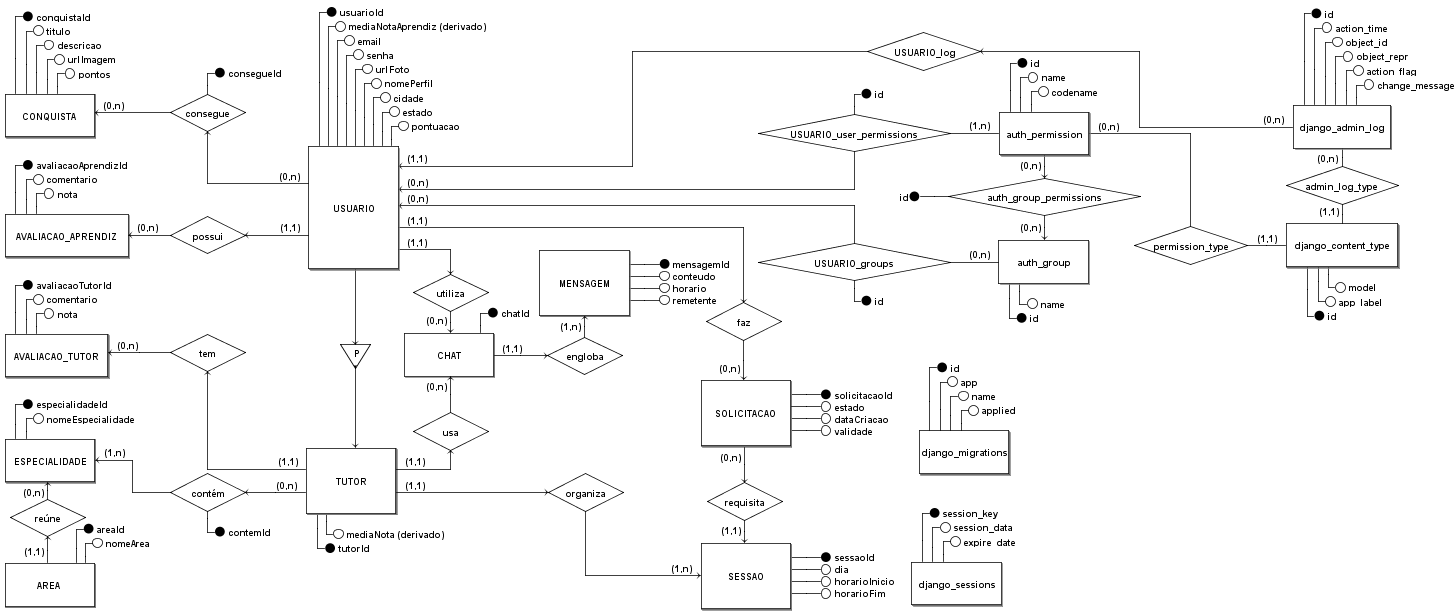
\includegraphics[width=1.5\textwidth, height=0.90\textheight, keepaspectratio]{figuras/DE-R.png}
    
    
        Fonte: Autoria própria.
        
        \vspace{0.2cm}
            
        \label{fig:diagrama_DE-R}
    \end{figure}
\end{landscape}

\clearpage

\subsection[Diagrama Lógico de Dados]{Diagrama Lógico de Dados}

O nível lógico de um projeto de banco de dados é uma descrição da base de dados que será implementada no Sistema Gerenciador de Banco de Dados (SGBD). Assim, cada entidade do banco é traduzida para uma tabela, e cada atributo, geralmente, define uma coluna desta tabela. Além disso, definem-se as chaves primárias e chaves estrangeiras,  os tipos de dados de cada coluna, dentre outros
recursos e restrições relevantes a base de dados que estará sendo implementada \cite{heuser2009projeto}. A Figura \ref{fig:diagrama_DLD} apresenta o Diagrama Lógico de Dados (DLD) do projeto.

Além do DLD e DE-R, foi criado um dicionário de dados da base de dados do software proposto. Um dicionário de dados é a descrição da base de dados, armazenando informações sobre sua estrutura e restrições \cite{elmasri2011sistemas}. No  Apêndice \ref{dicionario-dados} pode ser observado tal dicionário. 

\clearpage

\begin{landscape}
    \begin{figure}[h!]
        \centering
        \caption{Diagrama Lógico de Dados.} 
        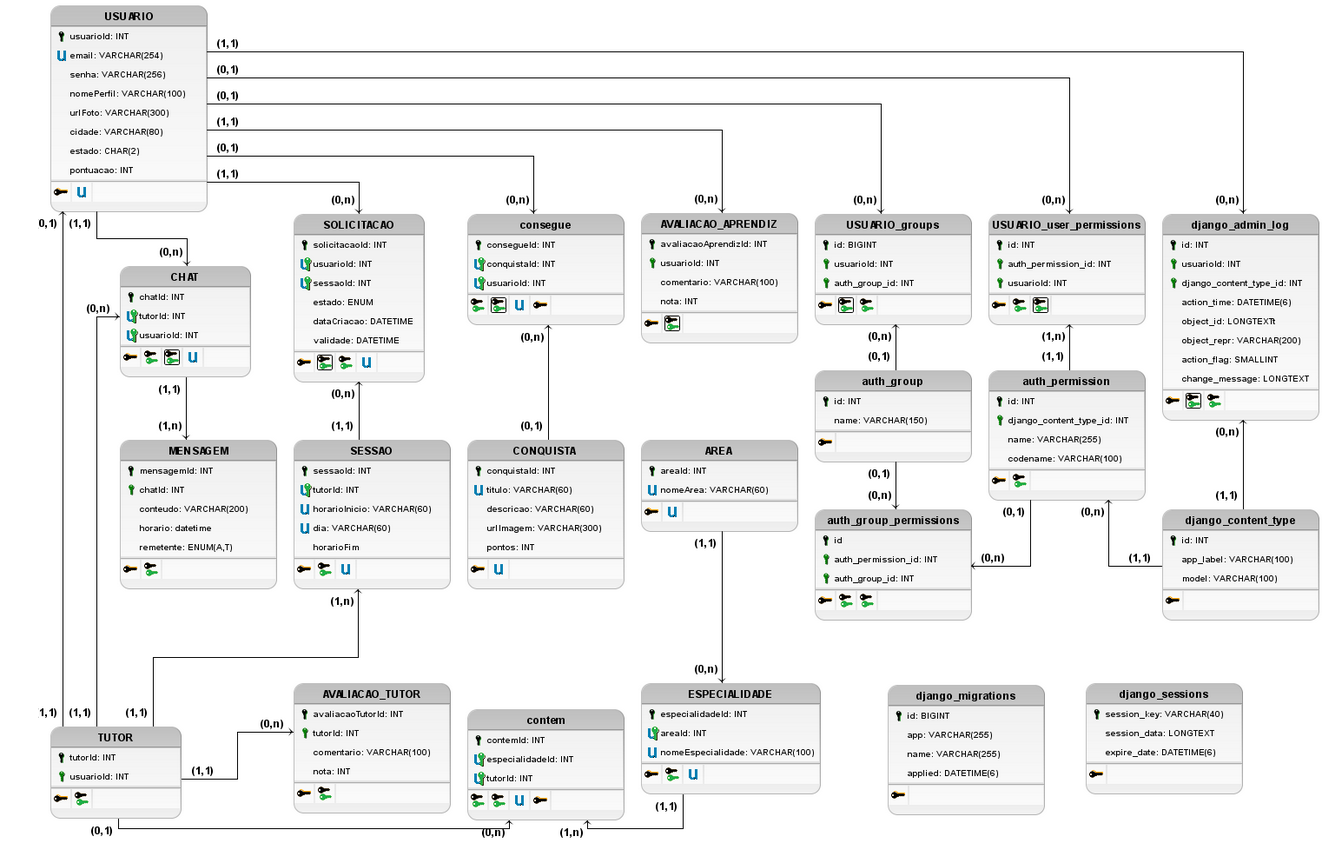
\includegraphics[width=1.5\textwidth, height=0.90\textheight, keepaspectratio]{figuras/DLD_print.png}
    
    
        Fonte: Autoria própria.
        
        \vspace{0.2cm}
            
        \label{fig:diagrama_DLD}
    \end{figure}
\end{landscape}

\clearpage

\section[Suporte Tecnológico]{Suporte Tecnológico}

Para auxiliar o processo de desenvolvimento deste projeto, foram utilizadas as ferramentas tecnológicas descritas a seguir:

\subsection[Git]{Git}
O Git é um sistema de controle de versão distribuído, gratuito e de código aberto, projetado para lidar com projetos de todos os tamanhos com velocidade e eficiência \cite{git2026}. O Git permite que cada desenvolvedor tenha uma cópia completa do histórico do projeto.

Neste trabalho, o Git foi utilizado para o versionamento de todo o código-fonte da simulação e do software, permitindo o controle das alterações e a integridade do trabalho desenvolvido.

\subsection[GitHub]{GitHub}
O GitHub é uma plataforma de hospedagem de código-fonte que utiliza o sistema Git para controle de versão, oferecendo também ferramentas de colaboração e gerenciamento de projetos \cite{github2026}. Ele atua como um ponto central para o armazenamento do repositório remoto.

No contexto deste projeto, o GitHub foi utilizado para hospedar os repositórios do \textit{frontend} e \textit{backend}, facilitando a colaboração entre os desenvolvedores e o acompanhamento das atualizações do código.

\subsection[brModelo]{brModelo}
O brModelo é uma ferramenta CASE (\textit{Computer-Aided Software Engineering}) de código aberto, voltada para o ensino e a modelagem de bancos de dados relacionais \cite{candido2020brmodelo}. Ela permite a criação de modelos conceituais e lógicos de maneira intuitiva.

Para este projeto, a ferramenta foi empregada na elaboração do DE-R e do DLD.

\subsection[Canva]{Canva}
O Canva é uma plataforma de design gráfico e comunicação visual online que oferece ferramentas para a criação de diversos tipos de conteúdos visuais, como apresentações, infográficos e diagramas \cite{canva2026}.

Neste trabalho, o Canva foi utilizado para a criação do diagrama ilustrativo da arquitetura do projeto.

\subsection[LaTeX e Overleaf]{LaTeX e Overleaf}

O LaTeX é um sistema de preparação de documentos de alta qualidade tipográfica, amplamente utilizado para a produção de documentação técnica e científica, facilitando a gestão de referências bibliográficas e fórmulas matemáticas \cite{latex2026}. O Overleaf, por sua vez, é uma ferramenta de edição e publicação colaborativa online baseada em LaTeX \cite{overleaf2026}.

A escolha dessas ferramentas para a escrita desta monografia deve-se à facilidade de formatação conforme as normas acadêmicas, à gestão automatizada de referências e à capacidade de edição simultânea e colaborativa do documento pelos autores.

\subsection[Discord]{Discord}
Um aplicativo de comunicação gratuito que permite conversas por voz, vídeo e texto \cite{pearson2025discord}. Foi utilizado para a realização de reuniões com compartilhamento de tela para discussões e desenvolvimento do trabalho.

\subsection[Telegram]{Telegram}
Aplicativo de mensagens gratuito baseado em nuvem com suporte a chamadas de voz e vídeo, além de compartilhamento de arquivos \cite{telegram2025}. Utilizado para comunicação, reuniões de acompanhamento de progresso entre os desenvolvedores e compartilhamento de arquivos.

\subsection[LucidChart]{LucidChart}
O Lucidchart é uma ferramenta baseada na web que auxilia usuários na criação e compartilhamento de fluxogramas, diagramas e mapas mentais profissionais de forma colaborativa \cite{lucidchart}. A plataforma permite a construção visual de processos complexos de maneira intuitiva.

Neste trabalho, o Lucidchart foi utilizado para a elaboração dos diagramas de fluxo de atividades dos processos metodológicos, permitindo a visualização clara das etapas de desenvolvimento do projeto.

\section[Processo Metodológico]{Processo Metodológico}

O Trabalho de Conclusão de Curso (TCC) em curso de Engenharia de Software na Universidade de Brasília (UnB) é realizado em duas etapas, denominadas TCC1 e TCC2. No TCC1 o objetivo é buscar o embasamento teórico necessário do projeto, bem como a elaboração de uma proposta de projeto. No TCC2 realiza-se a execução do planejamento elaborado na etapa anterior, consistindo no desenvolvimento completo das funcionalidades do software, na aplicação de testes e, por fim, na análise dos resultados alcançados para averiguar o êxito da solução proposta.

Com o propósito de definir e acompanhar o processo de desenvolvimento completo do TCC, foi modelado um processo metodológico para cada etapa, apresentados nas Seções \ref{sec:tcc1} e \ref{sec:tcc2}, além dos respectivos cronogramas com suas principais atividades.

\subsection[TCC1]{TCC1}
\label{sec:tcc1}

Nesta seção, é detalhado o processo metodológico adotado para a condução da primeira etapa do trabalho (TCC1). O fluxo de atividades realizadas é ilustrado na Figura \ref{fig:metodologiaTCC1}. A seguir, são descritas as atividades que compõem esse fluxo, bem como o cronograma de execução das atividades.

\begin{figure}[h!]
    \centering
    \caption{Metodologia para elaboração do TCC1.} 
    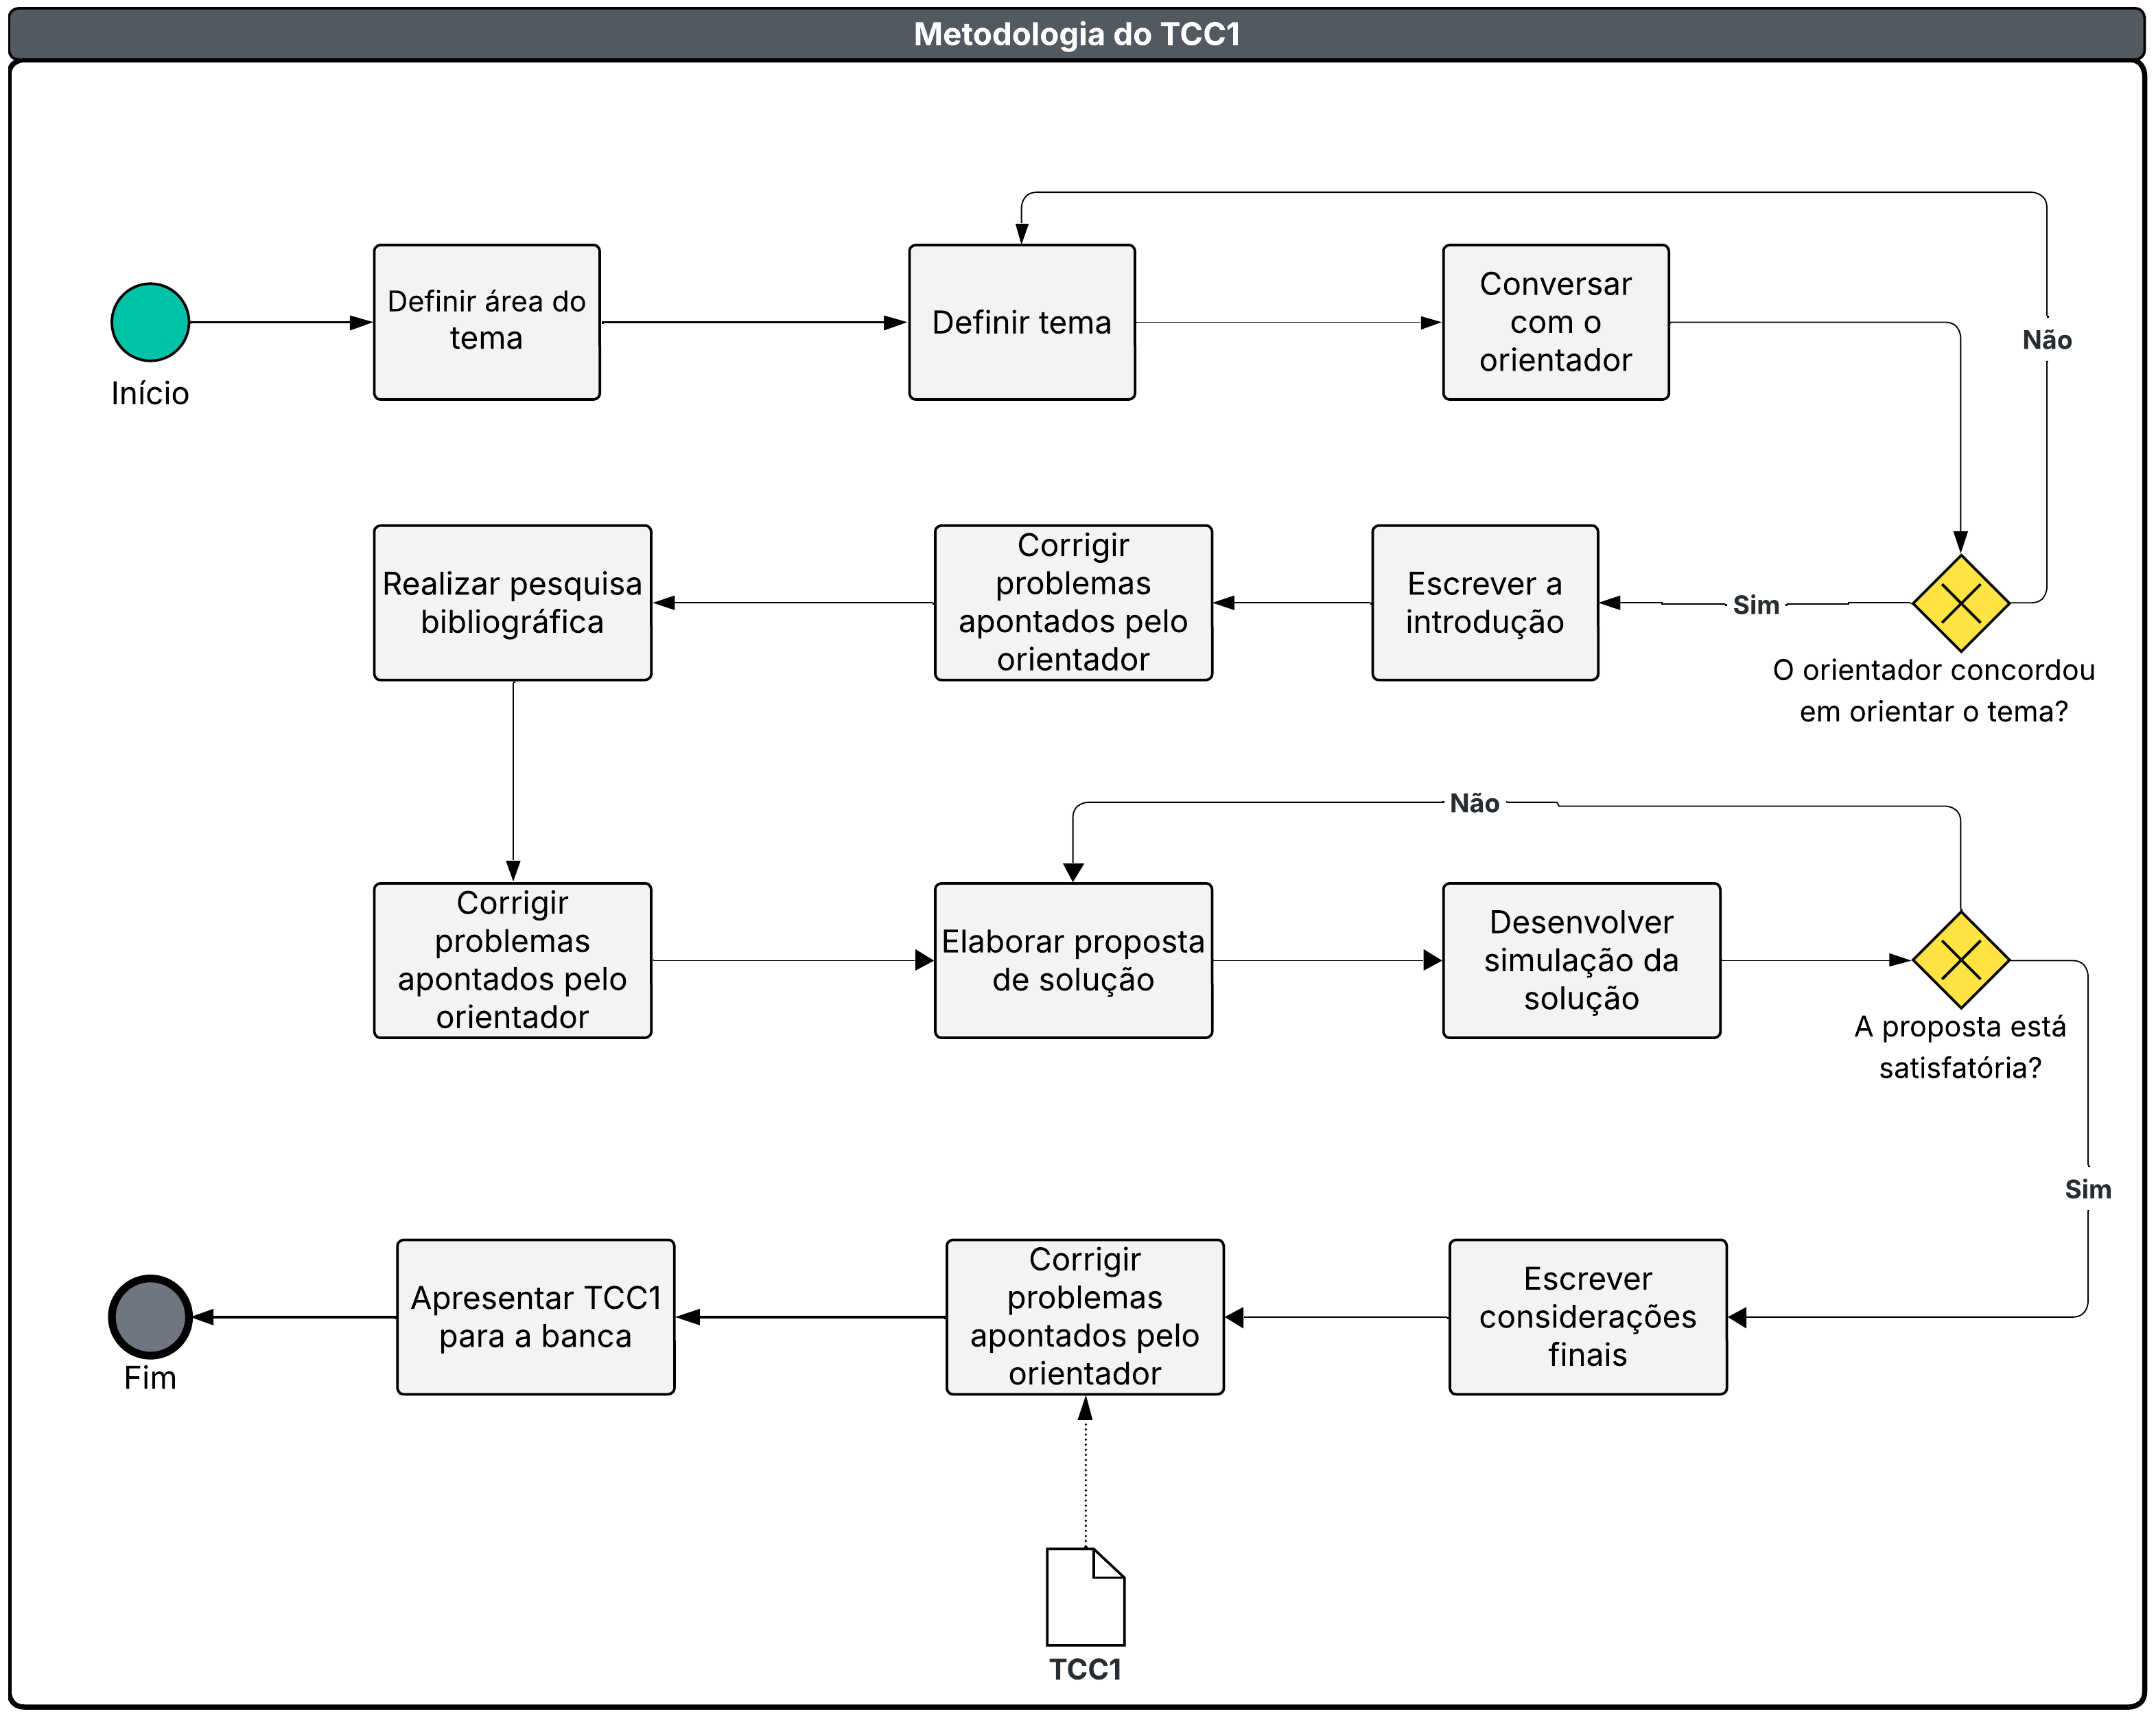
\includegraphics[width=0.87\textwidth]{figuras/diagrama_atividades_TCC1.png}


    Fonte: Autoria própria.
    
    \vspace{0.2cm}
        
    \label{fig:metodologiaTCC1}
\end{figure}

As atividades presentes na Figura \ref{fig:metodologiaTCC1} são descritas a seguir:

\begin{itemize}

\item \textbf{Definir área do tema}: definir qual área de Engenharia da Software será empregada no trabalho;

\item \textbf{Definir tema}: dentro da área escolhida, definir qual será o tema principal a ser desenvolvido no trabalho;

\item \textbf{Conversar com o orientador}: conversar com o orientador para validar o tema e verificar sua disponibilidade e interesse em orientar o trabalho proposto no TCC;

\item \textbf{Escrever a introdução}: detalhar o contexto do projeto proposto;

\item \textbf{Corrigir problemas apontados pelo orientador}: corrigir e evoluir todos os apontamentos indicados pelo orientador do trabalho;

\item \textbf{Realizar pesquisa bibliográfica}: pesquisar autores, artigos e publicações a respeito de temas relevantes para um melhor entendimento do trabalho trabalho e seu contexto;

\item \textbf{Elaborar proposta de solução}: apresentar a proposta de software a ser desenvolvida na primeira etapa do TCC;

\item \textbf{Desenvolver simulação da solução}: desenvolver parcialmente algumas funcionalidades do software proposto a fim de validar a viabilidade da arquitetura proposta, disponível no Apêndice X;

\item \textbf{Escrever considerações finais}: elaborar de maneira sucinta e objetiva o que foi alcançado com a proposta de trabalho (TCC1);

\item \textbf{Apresentar TCC1 para a banca}: realizar a apresentação da proposta para a banca examinadora.

\end{itemize}

\newpage

\subsubsection[Cronograma TCC1]{Cronograma TCC1}

\begin{table}[h!]
\centering
\caption{Cronograma com principais Atividades Previstas para o TCC1.}
\label{tab:cronograma-atividades-final}
\small 
\setlength{\tabcolsep}{4pt} 
\begin{tabular}{|l|c|c|c|c|c|c|c|c|c|c|c|c|}
\hline
\textbf{Atividade} & 
\rotatebox{90}{\textbf{Dezembro - 2024}} & 
\rotatebox{90}{\textbf{Janeiro - 2025}} & 
\rotatebox{90}{\textbf{Março - 2025}} & 
\rotatebox{90}{\textbf{Abril - 2025}} & 
\rotatebox{90}{\textbf{Maio - 2025}} & 
\rotatebox{90}{\textbf{Junho - 2025}} & 
\rotatebox{90}{\textbf{Julho - 2025}} & 
\rotatebox{90}{\textbf{Agosto - 2025}} & 
\rotatebox{90}{\textbf{Setembro - 2025}} &
\rotatebox{90}{\textbf{Outubro - 2025}} &
\rotatebox{90}{\textbf{Novembro - 2025}} &
\rotatebox{90}{\textbf{Dezembro - 2025}} \\
\hline \hline
\textbf{Definir área do tema} & X & & & & & & & & & & & \\ \hline
\textbf{Definir tema} & X & & & & & & & & & & & \\ \hline
\textbf{Conversar com o orientador} & X & & & & & & & & & & & \\ \hline
\textbf{Corrigir problemas apontados pelo orientador} & & & & & & X & X & & & & X & \\ \hline
\textbf{Escrever a introdução} & X & X & & & & & & & & & & \\ \hline
\textbf{Realizar pesquisa bibliográfica} & & & X & X & X & & & & & & & \\ \hline
\textbf{Elaborar proposta de solução} & & & & & & X & X & X & X & X & & \\ \hline
\textbf{Desenvolver simulação da solução} & & & & & & & & & & X & & \\ \hline
\textbf{Escrever considerações finais} & & & & & & & & & & & X & \\ \hline
\textbf{Apresentar TCC1 para a banca} & & & & & & & & & & & & X \\ \hline
\end{tabular}
\par
\vspace{2mm}
Fonte: Autoria própria.
\end{table}

Embora a disciplina de TCC1 seja prevista para um semestre letivo, a elaboração deste trabalho estendeu-se pelo período de um ano. Essa extensão de prazo foi necessária para permitir uma investigação bibliográfica mais exaustiva, visando consolidar um embasamento teórico robusto para os capítulos iniciais, diante da especificidade dos temas abordados. Adicionalmente, houve a necessidade de readequar o cronograma para conciliar o desenvolvimento da proposta com a carga acadêmica das demais disciplinas cursadas simultaneamente, garantindo assim a qualidade da entrega final.

\subsection[TCC2]{TCC2}
\label{sec:tcc2}

Nesta seção, é detalhado o processo metodológico adotado para o desenvolvimento da segunda etapa do trabalho (TCC2). O fluxo de atividades realizadas é ilustrado na Figura
\ref{fig:metodologiaTCC2}. A seguir, são descritas as atividades que compõem esse fluxo, bem como o cronograma elaborado para a execução das atividades e o plano de testes elaborado para o software desenvolvido.

\newpage

\begin{figure}[h!]
    \centering
    \caption{Metodologia para elaboração do TCC2.} 
    
    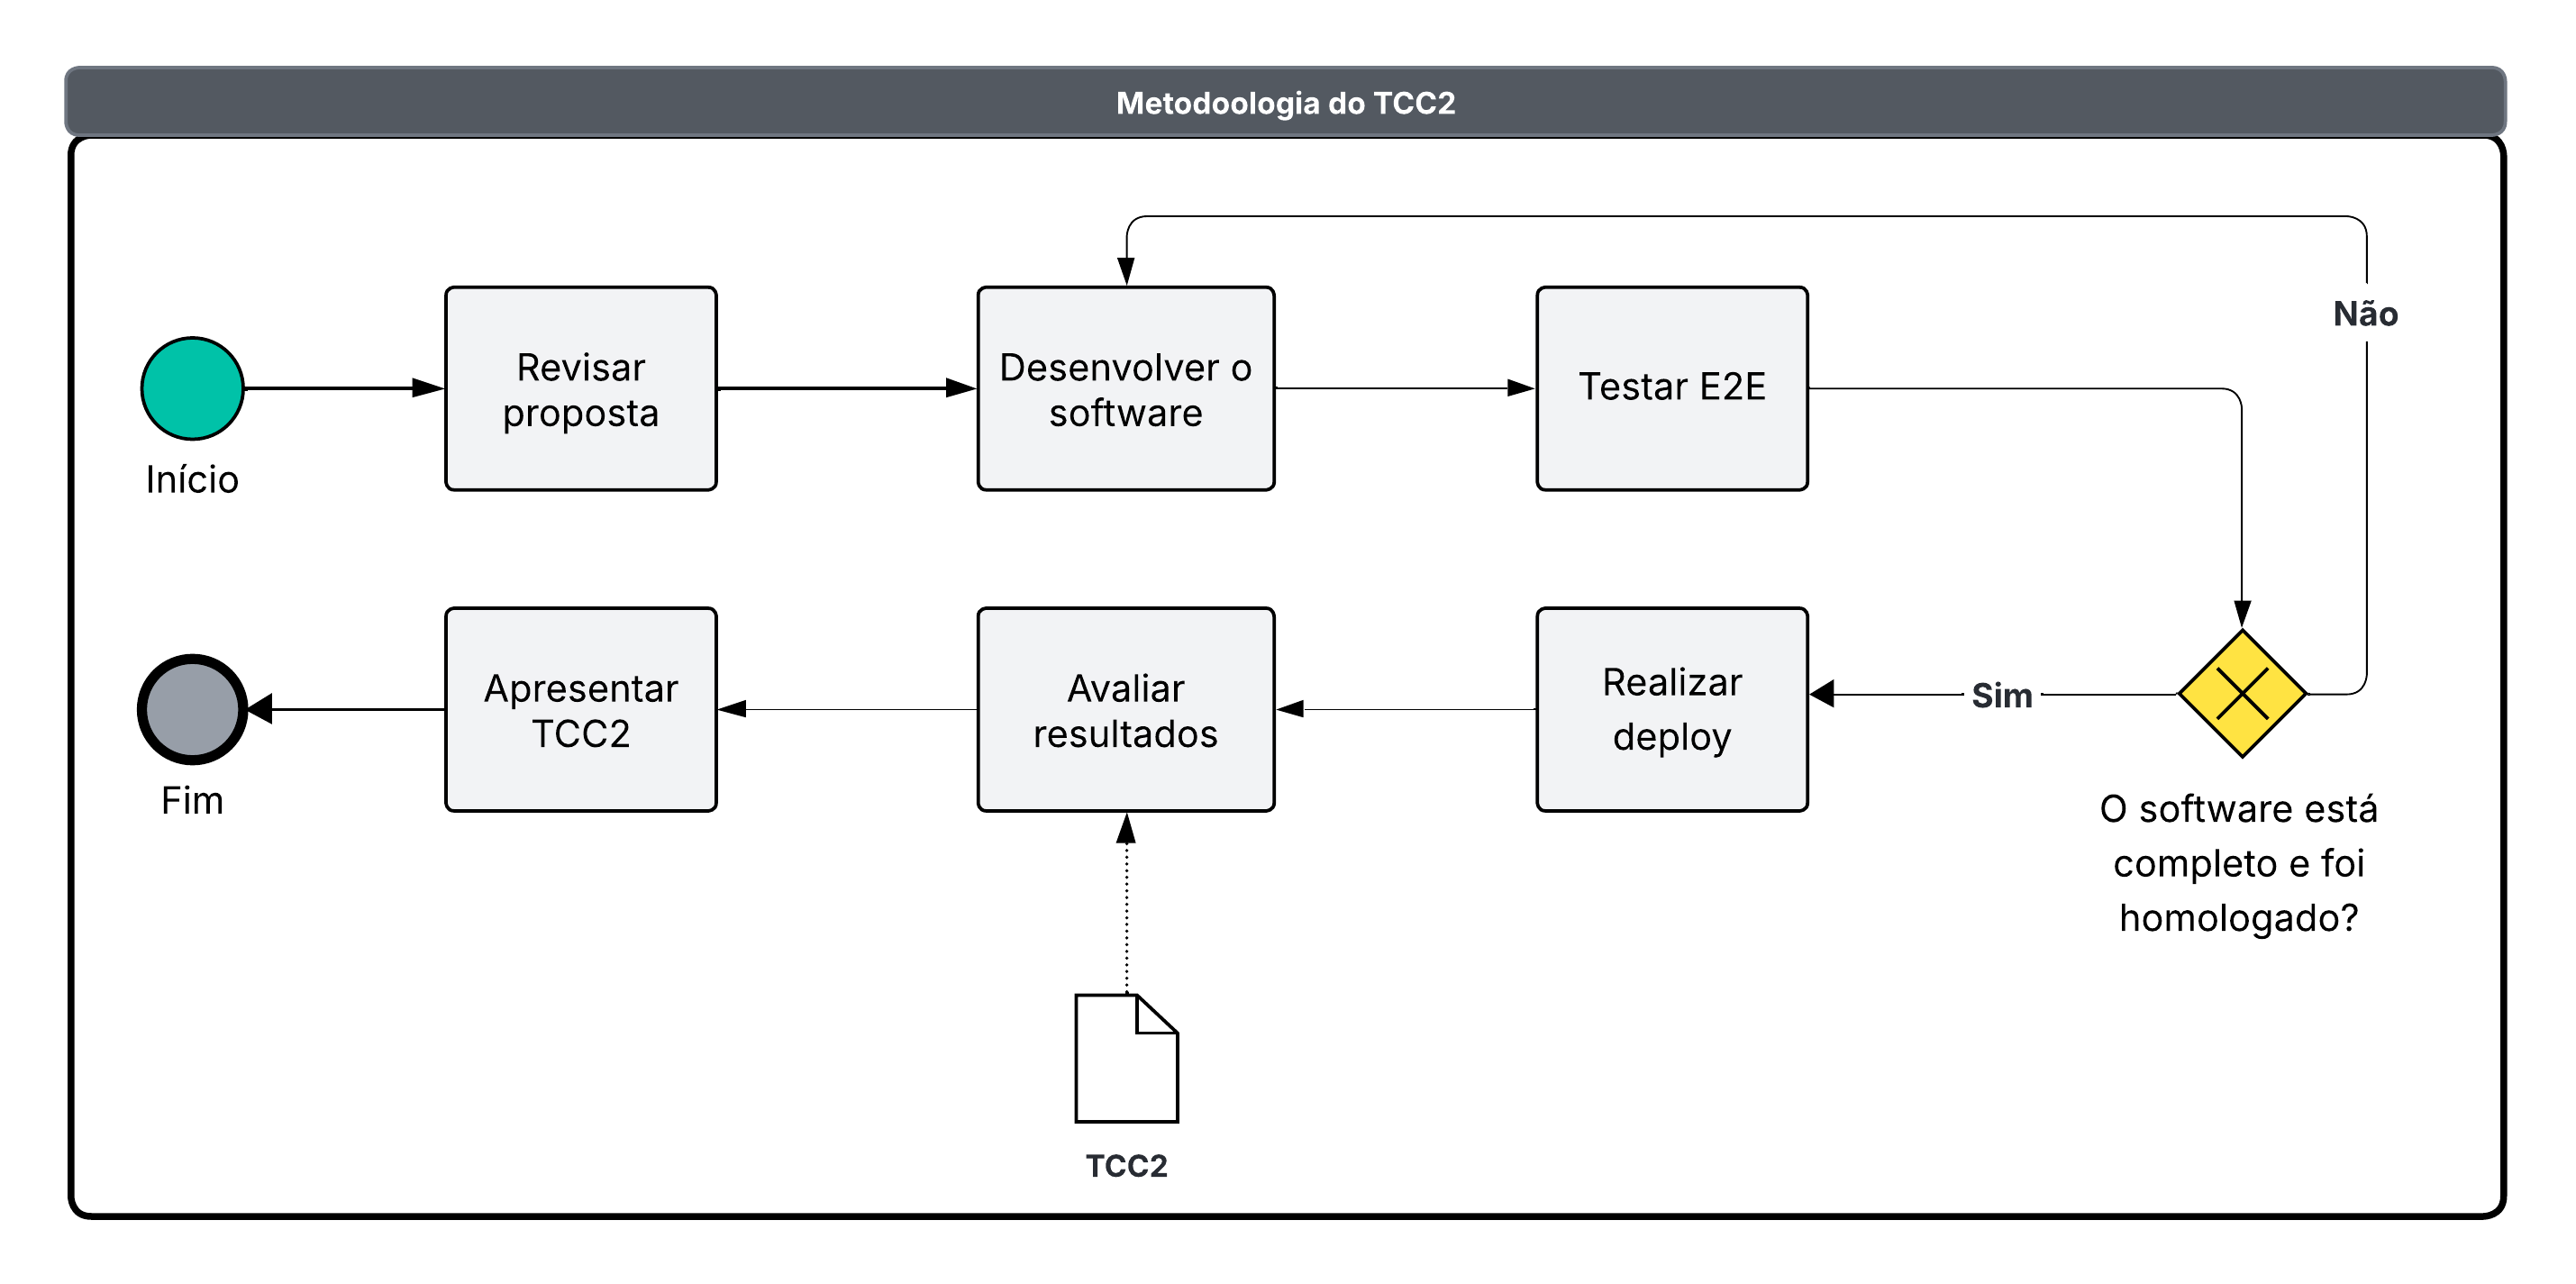
\includegraphics[width=0.90\textwidth]{figuras/diagrama_atividades_TCC2.png}
    
    \vspace{0.2cm}

    
    Fonte: Autoria própria.
    
    \label{fig:metodologiaTCC2}
\end{figure}

As atividades presentes na Figura \ref{fig:metodologiaTCC2} são descritas a seguir:

\begin{itemize}

\item \textbf{Revisar proposta}: realizar adições ou modificações no conteúdo do trabalho conforme o \textit{feedback} dos professores da banca avaliadora após a apresentação do TCC1;

\item \textbf{Desenvolver o software}: elaborar as funcionalidades do software seguindo a metodologia de desenvolvimento em conjunto com a realização de testes unitários e de integração conforme o plano de testes elaborado descrito na Subseção \ref{sec:PlanoDeTestes};

\item \textbf{Testar E2E}: realizar os testes End-to-End (E2E) para identificar inconsistências no fluxo de trabalho do usuário, visando a validação e homologação do software.

\item \textbf{Realizar \textit{deploy}}: realizar o \textit{deploy} do \textit{backend} e \textit{frontend} do software, possibilitando sua utilização pelos perfis de usuário através da Internet;

\item \textbf{Avaliar resultados}: analisar criticamente o software final desenvolvido, comparando os resultados alcançados com os objetivos propostos no trabalho e elaborar as conclusões finais do trabalho;

\item \textbf{Apresentar o TCC2}: realizar a apresentação do projeto para a banca examinadora.

\end{itemize}

\newpage

\subsubsection[Cronograma TCC2]{Cronograma TCC2}

\begin{table}[h!]
\centering
\caption{Cronograma de Atividades Previstas para o TCC2.}
\label{tab:cronograma-atividades-corrigido}
\small
\setlength{\tabcolsep}{4pt}
\begin{tabular}{|l|c|c|c|c|}
\hline
\textbf{Atividade} & \textbf{Março} & \textbf{Abril} & \textbf{Maio} & \textbf{Junho} \\ 
\hline \hline
Revisar proposta & X & & & \\ 
\hline
Desenvolver o software & X & X & X &  \\ 
\hline
Testar E2E & & & & X  \\ 
\hline
Realizar \textit{deploy} & & & & X  \\ 
\hline
Avaliar resultados & & & & X \\ 
\hline
Apresentar o TCC2 & & & & X \\ 
\hline
\end{tabular}
\par\vspace{2mm}
 Fonte: Autoria própria.
\end{table}

Conforme mencionado na subseção \ref{metodologia-desenvolvimento}, os ciclos de trabalho foram de uma semana. Sendo assim, as US listadas na subseção \ref{historias-usuario} estão distribuídas pelo cronograma da seguinte maneira:

\begin{itemize}

\item \textbf{Semana 1 (08-14 de Março)}: US01 (\textit{Login}) e US02 (Recuperar Senha);

\item \textbf{Semana 2 (15-21 de Março)}: US03 (Alterar Senha) e US04 (Alterar Informações);

\item \textbf{Semana 3 (22-28 de Março)}: US05 (Definir Agenda) e US06 (Gerenciar Especialidades).

\item \textbf{Semana 4 (29 de Março - 04 de Abril)}: US07 (Solicitar Horário);

\item \textbf{Semana 5 (05-11 de Abril)}: US08 (Aceitar e Recusar Solicitação) e US09 (Expirar Solicitação);

\item \textbf{Semana 6 (12-18 de Abril)}: US14 (Buscar Tutores);

\item \textbf{Semana 7 (19-25 de Abril)}: US10 (Avaliar Tutor);

\item \textbf{Semana 8 (26 de Abril - 02 de Maio)}: US11 (Avaliar Aprendiz) e US12 (Ver Reputação no Perfil);

\item \textbf{Semana 9 (03-09 de Maio)}: US13 (Enviar Mensagem);

\item \textbf{Semana 10 (10-16 de Maio)}: US15 (Recomendações);

\item \textbf{Semana 11 (17-23 de Maio)}: US16 (Conquistas);

\item \textbf{Semana 12 (24-30 de Maio)}: US17 (Níveis) e US18 (Títulos);

\end{itemize}

\subsubsection[Plano de Testes]{Plano de Testes}
\label{sec:PlanoDeTestes}

O plano de testes para o TCC 2 é realizar o TDD (do inglês \textit{Test Driven Development}, Desenvolvimento Orientado a Teste) com uma pirâmide de testes que abrange as funcionalidades descritas na Subseção \ref{historias-usuario}. A abordagem escolhida para o TDD é a Comportamental, que foca a validação apenas nos métodos públicos e fluxos principais. 

O projeto priorizou a validação por comportamento, assegurando que os testes cubram as regras de negócio relevantes e contratos de interface, evitando o acoplamento excessivo aos detalhes de implementação interna.

Os testes contemplam os níveis de teste unitário, teste de integração e teste E2E, que serão descritos a seguir:

\begin{itemize}

\item \textbf{Teste Unitários}: Técnica de teste automatizado que verifica as menores partes de um código, como funções ou métodos, isoladamente. O projeto tem uma cobertura de código de 70\% de testes unitários.

\item \textbf{Testes de Integração}: Utilizando abordagem ampla e \textit{Top-Down} de teste de integração, que inicia a validação na camada de interface mais alta (API/\textit{Endpoints}) e segue hierarquicamente até as camadas inferiores de infraestrutura e persistência.

O objetivo é simular o comportamento real de consumo do serviço, garantindo que a comunicação flua corretamente desde a entrada da requisição até a resposta dos componentes externos reais, validando a integridade da pilha completa de execução.

% Verifica a comunicação e a interação entre diferentes módulos ou componentes de um software, combinando-os para garantir que funcionem corretamente juntos. Serão executados testes de integração em todos os endpoints. Os testes unitários serão responsáveis por guiar o design da arquitetura interna, validando a existência de classes, métodos e regras de negócio. Enquanto os testes de integração focarão na validação dos \textit{endpoints} das funcionalidades, assegurando que os contratos da API e o fluxo de dados entre os componentes respondam corretamente às requisições.

\item \textbf{Teste E2E}: Simula o fluxo de trabalho de um usuário real com o sistema desenvolvido, para validar a aplicação do início ao fim, garantindo que todos os componentes integrados funcionem corretamente juntos. Foram aplicados testes E2E nas páginas em que haja interação com o usuário, evitando-se as páginas de somente exibição de texto.

\end{itemize}

\subsubsubsection[Ferramentas de Teste]{Ferramentas de Teste}
\begin{itemize}
    \item \textbf{POSTMAN}: Ferramenta para realização de testes de API.
    \item \textbf{DjangoUnit}: \textit{Framework} Python utilizado para teste unitários na \textit{Framework} Django.
    \item \textbf{Robot}: \textit{Framework} Python utilizada para testes E2E em aplicações web.
\end{itemize}

\subsubsubsection[Classificação de Bugs]{Classificação de Bugs}
Os \textit{bugs} estão classificados com as seguintes severidades descritas na Tabela \ref{tab:classificacao-bugs}.

\newpage

\begin{table}[h!]
    \centering
    \caption{Classificação dos \textit{Bugs}.}
    \label{tab:classificacao-bugs}
    % Define a tabela para ocupar 100% da largura da linha (\linewidth)
    % A coluna X se ajusta automaticamente para preencher o espaço restante
    \begin{tabularx}{\linewidth}{|c|l|X|}
        \hline
        \textbf{ID} & \textbf{Nível de Severidade} & \textbf{Descrição} \\
        \hline
        1 & Pequena & 
        \begin{itemize}
            \item Quase nenhum impacto na funcionalidade, porém atrapalha a experiência do usuário.
            \item Pequenos erros de interface do usuário.
            \item Erro ortográfico.
        \end{itemize}
        \\
        \hline
        2 & Moderada & 
        \begin{itemize}
            \item Funcionalidade não atinge certos critérios de aceitação, mas não compromete sua funcionalidade em geral.
        \end{itemize}
        \\
        \hline
        3 & Grave &
        \begin{itemize}
            \item Funcionalidade não funciona como o esperado.
            \item Interação de usuário incomum causa efeitos irreversíveis e prejudiciais.
        \end{itemize}
        \\
        \hline
        4 & Severa &
        \begin{itemize}
            \item Bug que bloqueia o teste de uma função ou causa falha na aplicação.
            \item Redirecionamento de página ou eventos de botão que impedem o uso da funcionalidade.
        \end{itemize}
        \\
        \hline
    \end{tabularx}
    \vspace{0.2cm} % Um pequeno espaço antes da fonte
    
    Fonte: Autoria Própria.
\end{table}

\subsubsubsection[Definição de Pronto]{Definição de Pronto}
Foi considerada pronta a funcionalidade que passou pela verificação de testes descrita e não apresentou \textit{bugs} com  severidade acima de Pequena ou não existiu \textit{bug} para esta funcionalidade.